\section{Simulation Analysis}
\label{sec:simulation}
In this section we will describe the steps needed to simulate this circuit using the software Ngspice.Three types of analysis will be performed:Operating Point analysis, Transient analysis ans Frequency analysis.

The following steps in the simulations are to be conducted: 
\begin{itemize}
	\item for $t<0$ (operating point only, in order to obtain the voltages in all nodes and the currents in all branches);
	\item operating point for  $V_s(0) = 0$, replacing the capacitor with a a voltage source $V_x = V_6-V_8$, where $V_6$ and $V_8$ are the voltages in nodes 6 and 8 as obtained in the previous step (this step is necessary given that we must the compute the boundary conditions that guarantee continuity in the capacitor's discharge - such may imply that the boundary conditions differ from those computed for t<0);
	\item simulate the natural response of the circuit (using the boundary conditions V(6) and V(8) as obtained previously) using a transient analysis;
	\item repeating the third step, using {\it $V_s$} as given in \textbf{Figure~\ref{fig:time_step}} and f = 1kHz  in order to simulate for the total response on node 6
	\item simulate the frequency response in node 6 for a frequency range 0.1 Hz to 1MHz.
\end{itemize}
 
 \begin{figure}[H] \centering
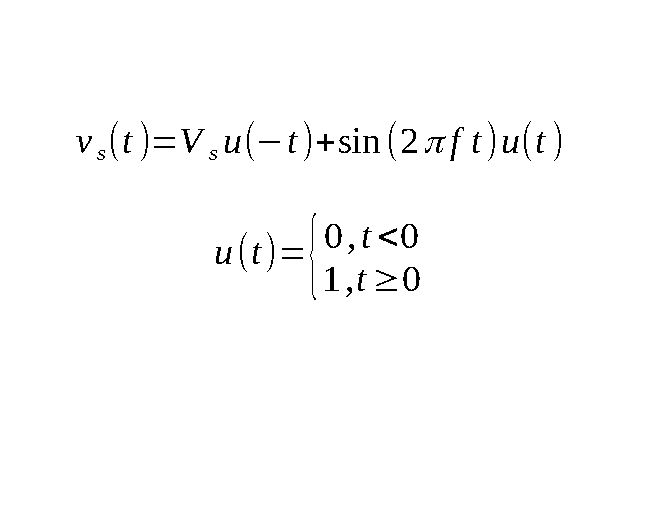
\includegraphics[width=0.5\linewidth]{time_step.pdf}
\caption{Time step conditions}
\label{fig:time_step}
\end{figure}

\subsection{Operating Point Analysis for $t<0$}
There was a need to create a "fictional" voltage source, between node 7 and resistor 6 (providing 0V to the circuit in order not to alter the behaviour of the rest of the circuit) so as to be able to define the dependecy for the current-controlled voltage source {\it $V_d$}. This has no specific reason to be, other than the particularities of the Ngspice software. THe circuit and nodes used for the simulation can be seen in \textbf{Figure~\ref{fig:diagram_t2}}.\par 
\textbf{Table~\ref{tab:op}} shows the simulated operating point results for the circuit
under analysis for $t<0$. 
%The current flows considered in the theoretical section were coherent with the polarity implicitly declared when defining the circuit to be simulated in the Ngspice script.\par

\begin{table}[h!]
  \centering
  \begin{tabular}{|l|r|}
    \hline    
    {\bf Name} & {\bf Value [mA or V]} \\ \hline
    @c[i] & 0.000000e+00\\ \hline
@gb[i] & -2.91567e-04\\ \hline
@r1[i] & 2.780494e-04\\ \hline
@r2[i] & 2.915672e-04\\ \hline
@r3[i] & -1.35178e-05\\ \hline
@r4[i] & -1.22689e-03\\ \hline
@r5[i] & -2.91567e-04\\ \hline
@r6[i] & 9.488377e-04\\ \hline
@r7[i] & 9.488377e-04\\ \hline
v(1) & 5.243596e+00\\ \hline
v(2) & 4.952739e+00\\ \hline
v(3) & 4.367468e+00\\ \hline
v(4) & -1.96340e+00\\ \hline
v(5) & 4.994112e+00\\ \hline
v(6) & 5.904536e+00\\ \hline
v(7) & -1.96340e+00\\ \hline
v(8) & -2.92677e+00\\ \hline

  \end{tabular}
  \caption{Step 1: Operating point for t<0. A variable preceded by @ is of type {\em current}
    and expressed in miliAmpere; other variables are of type {\it voltage} and expressed in
    Volt.}
  \label{tab:op}
\end{table}

%tabela correspondente ao ponto 2) do simulation analysis
\pagebreak
\subsection{Operating Point Analysis for $t=0$}

\begin{table}[h!]
  \centering
  \begin{tabular}{|l|r|}
    \hline    
    {\bf Name} & {\bf Value [mA or V and Ohm]} \\ \hline
    @gb[i] & 4.151983e-18\\ \hline
@r1[i] & -3.95949e-18\\ \hline
@r2[i] & -4.15198e-18\\ \hline
@r3[i] & 1.924970e-19\\ \hline
@r4[i] & -8.72784e-19\\ \hline
@r5[i] & -2.82826e-03\\ \hline
@r6[i] & 4.336809e-19\\ \hline
@r7[i] & -8.83871e-19\\ \hline
v(1) & 0.000000e+00\\ \hline
v(2) & 4.141871e-15\\ \hline
v(3) & 1.247625e-14\\ \hline
v(4) & -8.97403e-16\\ \hline
v(5) & 3.552714e-15\\ \hline
v(6) & 8.831302e+00\\ \hline
v(7) & -8.97403e-16\\ \hline
v(8) & 0.000000e+00\\ \hline
Ix & -2.82826e-03\\ \hline
Vx & 8.831302e+00\\ \hline
Req & -3.12252e+03\\ \hline

  \end{tabular}
  \caption{Step 2: Operating point for {\it $v_s(0)=0$}, with the capacitor replaced by a voltage source {\it $V_x=V(6)-V(8)$} with these as obtained in the last step. A variable preceded by @ is of type {\em current}
    and expressed in miliAmpere; variables are of type {\it voltage} and expressed in
    Volt.The equivelant resistance is in Ohms}
  \label{tab:opeq}
\end{table}

\pagebreak
\subsection{ Natural solution for $V_6$ using transient analysis}
\begin{figure}[h] \centering
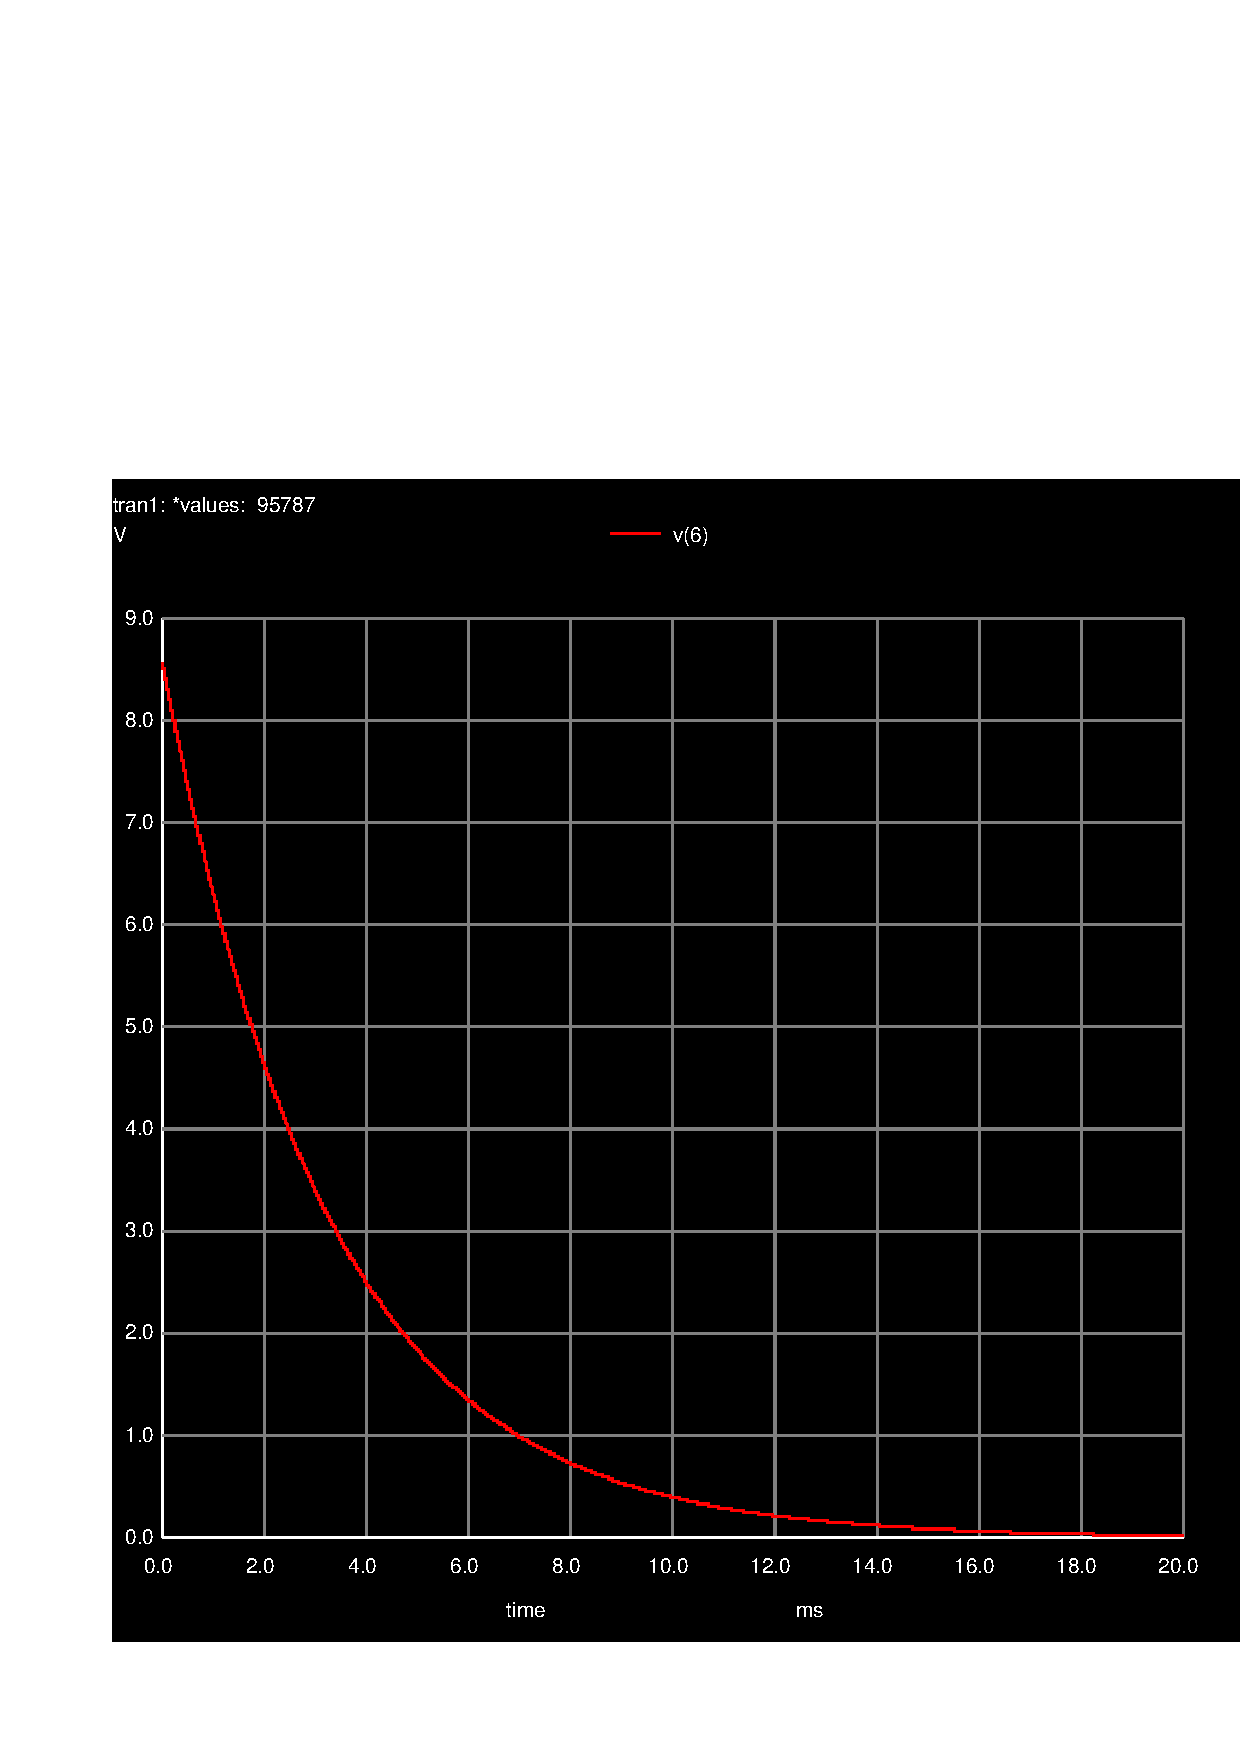
\includegraphics[width=0.6\linewidth]{trans.pdf}
\caption{estudo tranisiente}
\label{fig:transient}
\end{figure}

\pagebreak
\subsection{ Total solution for $V_6$ using transient analysis}

\pagebreak
\subsection{ Frequency response in node 6}

